\documentclass[11pt,a4paper]{article}
\usepackage[T1]{fontenc}
\usepackage[utf8]{inputenc}
\usepackage[french]{babel}
\usepackage{lmodern}
\usepackage{amsmath,amssymb}
\usepackage[a4paper,margin=2.5cm,headheight=14pt]{geometry}
\usepackage{graphicx}
\graphicspath{{./}{../../FIG/}}
\usepackage{booktabs}
\usepackage[table]{xcolor}
\usepackage{array}
\usepackage{float}
\usepackage{caption}
\usepackage{titlesec}
\usepackage{fancyhdr}
\usepackage{enumitem}
\usepackage[hidelinks]{hyperref}

\definecolor{secblue}{HTML}{1F6FC5}
\definecolor{subgray}{HTML}{465A6E}
\definecolor{headrow}{HTML}{DCE6F1}
\definecolor{nsrow}{HTML}{FDF1D6}
\hypersetup{colorlinks=true,linkcolor=secblue,urlcolor=secblue,pdfauthor={Marouane Boutayeb},pdftitle={Analyse des Taxis de Chicago},pdfsubject={Data Analysis}}

\frenchsetup{StandardItemLabels=true,SmallCapsFigTabCaptions=false}
\setcounter{secnumdepth}{2}
\setcounter{tocdepth}{2}
\setlength{\parindent}{1.5em}
\setlength{\parskip}{3pt}
\linespread{1.12}
\emergencystretch=2em

\titleformat{\section}{\Large\bfseries\color{secblue}}{\thesection.}{0.5em}{}[{\color{secblue}\titlerule[0.6pt]}]
\titleformat{\subsection}{\large\bfseries\color{subgray}}{\thesubsection.}{0.5em}{}
\titleformat{\subsubsection}{\normalsize\bfseries}{}{0em}{}
\titlespacing*{\section}{0pt}{16pt}{8pt}
\titlespacing*{\subsection}{0pt}{12pt}{6pt}

\pagestyle{fancy}
\fancyhf{}
\fancyhead[L]{\small Analyse des Taxis de Chicago}
\fancyhead[R]{\small DATA ANALYSIS}
\fancyfoot[C]{\thepage}
\renewcommand{\headrulewidth}{0.4pt}

\newcommand{\thead}[1]{\textbf{#1}}
\newcommand{\headrowcolor}{\rowcolor{headrow}}

\captionsetup{font=small,labelsep=colon}

\begin{document}

%================= PAGE DE GARDE =================
\begin{titlepage}
\pagenumbering{gobble}
\fontfamily{put}\selectfont
\centering
\vspace*{1.6cm}
{\bfseries École Supérieure d'Ingénierie en Sciences Appliquées\par}
\vspace{0.25cm}
{\bfseries Ingénierie des Systèmes d'Information \& Intelligence Artificielle\par}
{\bfseries Data analytics\par}
\vspace{1.2cm}
\rule{\linewidth}{1.2pt}\\[-0.85em]\rule{\linewidth}{0.4pt}\\[1.1cm]
{\LARGE Projet : Les taxis à Chicago (US)\par}
\vspace{1.0cm}
\rule{\linewidth}{1.2pt}\\[-0.85em]\rule{\linewidth}{0.4pt}\\[0.6cm]
\begin{minipage}[t]{0.48\linewidth}
\raggedright
Réalisé par :\\[0.35cm]
Boutayeb Marouane\\[0.25cm]
BELFAKIR Abdelfettah\\[0.25cm]
ES-SAIDI Anass
\end{minipage}\hfill
\begin{minipage}[t]{0.42\linewidth}
\raggedleft
\vspace{0.65cm}
Encadré par : Pr. HDIOUD Ferdaous
\end{minipage}

\vspace{1.6cm}

\includegraphics[width=0.43\linewidth]{logo_esisa.png}

\vfill
A.U : 2025-2026
\vspace*{1.5cm}
\end{titlepage}

\pagenumbering{roman}
\tableofcontents
\thispagestyle{fancy}
\clearpage
\pagenumbering{arabic}

%================= 1 =================
\section{Introduction et Description du Sujet}

Ce projet s'inscrit dans le cadre du cours d'\textit{Analyse de Données}. Il porte sur l'étude des
courses de taxi de la ville de \textbf{Chicago} (Illinois, États-Unis), disponibles sur le portail officiel
\texttt{data.cityofchicago.org} (dataset \textit{Taxi Trips}, identifiant : \texttt{wrvz-psew}).

La base de données recense l'ensemble des courses effectuées par les taxis de la ville depuis 2013.
Les trois variables d'intérêt sont :
\begin{itemize}
  \item $P$ --- \textbf{Prix total} (\texttt{trip\_total}, en dollars \$) ;
  \item $D$ --- \textbf{Durée} (\texttt{trip\_seconds}, en secondes) ;
  \item $L$ --- \textbf{Longueur} (\texttt{trip\_miles}, en miles).
\end{itemize}

L'objectif est de répondre aux trois questions statistiques suivantes :
\begin{enumerate}
  \item Tester si la moyenne de $P$, $D$ et $L$ change significativement en 2021 par rapport à la période
        2013--2020 (test à $\alpha = 5\,\%$).
  \item Étudier la relation entre le prix $P$ et les variables $L$ et $D$ (corrélation et régression linéaire).
  \item Identifier une plage horaire de pointe et tester la corrélation linéaire entre $P$ et la plage horaire
        (nécessite les horodatages).
\end{enumerate}

%================= 2 =================
\section{Présentation du Dataset}

Les données utilisées dans ce projet proviennent du dataset public \textit{Chicago Taxi Trips}.
Cette base contient les informations des trajets de taxis effectués dans la ville de Chicago entre 2013 et 2023.
Les principales variables utilisées dans cette étude sont :
\begin{itemize}
  \item \texttt{trip\_total} : prix total de la course (tarif, pourboire, péages et suppléments) ;
  \item \texttt{trip\_seconds} : durée du trajet en secondes ;
  \item \texttt{trip\_miles} : distance parcourue en miles ;
  \item \texttt{trip\_start\_timestamp} : date et heure de départ ;
  \item \texttt{trip\_end\_timestamp} : date et heure d'arrivée.
\end{itemize}
Les horodatages sont exprimés en heure locale de Chicago et arrondis au quart d'heure.

\subsection{Collecte des données}

Les données ont été extraites de la table publique BigQuery, copie du portail Open Data de la ville
(script \texttt{PRE/01\_download.py}) :
\begin{center}\texttt{bigquery-public-data.chicago\_taxi\_trips.taxi\_trips}\end{center}

Le dataset original est extrêmement volumineux : il contient plusieurs centaines de millions de trajets
couvrant les années 2013 à 2023, pour une taille totale qui dépasse 20 Go. Le téléchargement complet était
difficile à cause :
\begin{itemize}
  \item des limitations de l'API ;
  \item des erreurs de type \texttt{Timeout} ;
  \item des temps de téléchargement très longs ;
  \item des limitations de mémoire et de stockage.
\end{itemize}

Afin de rendre les traitements statistiques réalisables dans des conditions raisonnables, un
\textbf{échantillonnage aléatoire} a été effectué : pour chaque année entre 2013 et 2023, environ 108\,000
trajets ont été tirés au hasard. Le dataset final est donc un sous-ensemble représentatif des données
originales, de taille exploitable pour les analyses statistiques en Python.

Les fichiers obtenus sont : \texttt{\{2013.csv, 2014.csv, \ldots, 2023.csv\}}. Chaque fichier contient les
colonnes \texttt{trip\_total}, \texttt{trip\_seconds}, \texttt{trip\_miles}, \texttt{trip\_start\_\allowbreak timestamp}
et \texttt{trip\_end\_timestamp}. Le nombre de lignes et la taille de chaque fichier sont présentés dans le
tableau~\ref{tab:fichiers}.

\begin{table}[H]
\centering
\caption{Nombre de lignes et taille des fichiers CSV par année}
\label{tab:fichiers}
\begin{tabular}{lrr}
\toprule
\headrowcolor \thead{Fichier} & \thead{Nombre de lignes} & \thead{Taille (Mo)} \\
\midrule
2013.csv & 108\,900 & 8{,}01 \\
2014.csv & 107\,740 & 8{,}19 \\
2015.csv & 107\,820 & 8{,}17 \\
2016.csv & 106\,920 & 8{,}20 \\
2017.csv & 107\,097 & 8{,}18 \\
2018.csv & 106\,907 & 8{,}19 \\
2019.csv & 106\,706 & 8{,}19 \\
2020.csv & 106\,676 & 8{,}18 \\
2021.csv & 106\,490 & 8{,}18 \\
2022.csv & 106\,388 & 8{,}20 \\
2023.csv & 106\,293 & 8{,}21 \\
\midrule
\textbf{Total} & \textbf{1\,177\,937} & \textbf{$\approx$ 90} \\
\bottomrule
\end{tabular}
\end{table}

%================= 3 =================
\section{Description et Prétraitement des Données}

\subsection{Préparation et fusion des données}

Avant tout traitement statistique, les 11 fichiers CSV ont été fusionnés en un seul fichier
\texttt{chicago\_taxi\_raw.csv} à l'aide du script \texttt{PRE/02\_fusion.py}. Une attention particulière a été
portée au \textbf{séparateur décimal} : les fichiers utilisent la virgule comme séparateur décimal (format
français), par exemple \texttt{"0,01"}. La conversion a été effectuée en lisant les colonnes numériques comme
chaînes de caractères, puis en remplaçant la virgule par un point avant la conversion numérique :

\begin{verbatim}
df[col] = df[col].str.replace(',', '.', regex=False)
df[col] = pd.to_numeric(df[col], errors='coerce')
\end{verbatim}

Une colonne \texttt{year} a également été ajoutée lors de la fusion pour identifier l'année d'origine de
chaque trajet.

\subsection{Étapes de prétraitement}

Le prétraitement est réalisé par le script \texttt{PRE/03\_preprocess.py} :
\begin{enumerate}
  \item \textbf{Chargement} : 11 fichiers CSV (2013--2023) fusionnés en \textbf{1\,177\,937 lignes} brutes.
  \item \textbf{Suppression des valeurs manquantes ou nulles} ($P \le 0$, $D \le 0$, $L \le 0$) :
        180\,216 lignes supprimées.
  \item \textbf{Filtres de plausibilité} : 15\,257 lignes supprimées. On ne conserve que les courses avec
        $P \ge 3{,}25$\,\$ (prise en charge minimale d'un taxi à Chicago), $D \ge 60$\,s, $L \ge 0{,}1$\,mile et
        une vitesse moyenne $L/D \le 80$\,mph. Ces filtres éliminent les erreurs de saisie (prix de 0,01\,\$,
        courses d'une seconde, vitesses impossibles).
  \item \textbf{Suppression des \textit{outliers}} par la méthode IQR (facteur $k = 3$) sur $P$, $D$ et $L$ :
        6\,525 lignes supprimées.
  \item \textbf{Variables dérivées} : heure de départ, numéro de plage horaire (0 à 5), libellé de la plage et
        durée en minutes.
  \item \textbf{Résultat final} : \textbf{975\,939 courses} valides.
  \item \textbf{Séparation} : 2013--2020 en ensemble de référence (692\,502 courses) et 2021 en ensemble test
        (94\,792 courses).
\end{enumerate}

\subsubsection{Méthode IQR}

Pour chaque variable $X$, on calcule $Q_1$ et $Q_3$, puis :
\[
  X \text{ conservé si } \quad Q_1 - 3\cdot\mathrm{IQR} \;\le\; X \;\le\; Q_3 + 3\cdot\mathrm{IQR}
  \qquad \text{avec} \quad \mathrm{IQR} = Q_3 - Q_1
\]
Les bornes supérieures obtenues sont 140{,}57\,\$ pour $P$, 5\,715\,s pour $D$ et 50{,}70\,miles pour $L$.
Les distributions étant très asymétriques, les bornes inférieures sont \textbf{négatives} : la méthode IQR
ne supprime donc aucune valeur trop petite, d'où la nécessité des filtres de plausibilité de l'étape~3.

\subsection{Statistiques descriptives}

Le tableau~\ref{tab:desc} présente les principales statistiques de $P$, $D$ et $L$ pour les deux
sous-ensembles après prétraitement.

\begin{table}[H]
\centering
\caption{Statistiques descriptives des variables $P$, $D$ et $L$ après prétraitement}
\label{tab:desc}
\begin{tabular}{llrrrr}
\toprule
\headrowcolor \thead{Variable} & \thead{Période} & \thead{$n$} & \thead{Moyenne} & \thead{Écart-type} & \thead{Médiane} \\
\midrule
$P$ (\$) & Référence (2013--2020) & 692\,502 & 29{,}04 & 19{,}54 & 22{,}50 \\
$P$ (\$) & Test (2021) & 94\,792 & 34{,}51 & 19{,}35 & 29{,}75 \\ \midrule
$D$ (s) & Référence (2013--2020) & 692\,502 & 1\,452{,}1 & 955{,}5 & 1\,260{,}0 \\
$D$ (s) & Test (2021) & 94\,792 & 1\,536{,}3 & 799{,}0 & 1\,405{,}0 \\ \midrule
$L$ (miles) & Référence (2013--2020) & 692\,502 & 8{,}34 & 6{,}98 & 5{,}90 \\
$L$ (miles) & Test (2021) & 94\,792 & 9{,}54 & 6{,}66 & 8{,}94 \\
\bottomrule
\end{tabular}
\end{table}

Les trois distributions sont asymétriques à droite (médiane inférieure à la moyenne). La distribution de $L$
présente un second mode autour de 17--18 miles, qui correspond aux trajets vers les aéroports.

\begin{figure}[H]
\centering
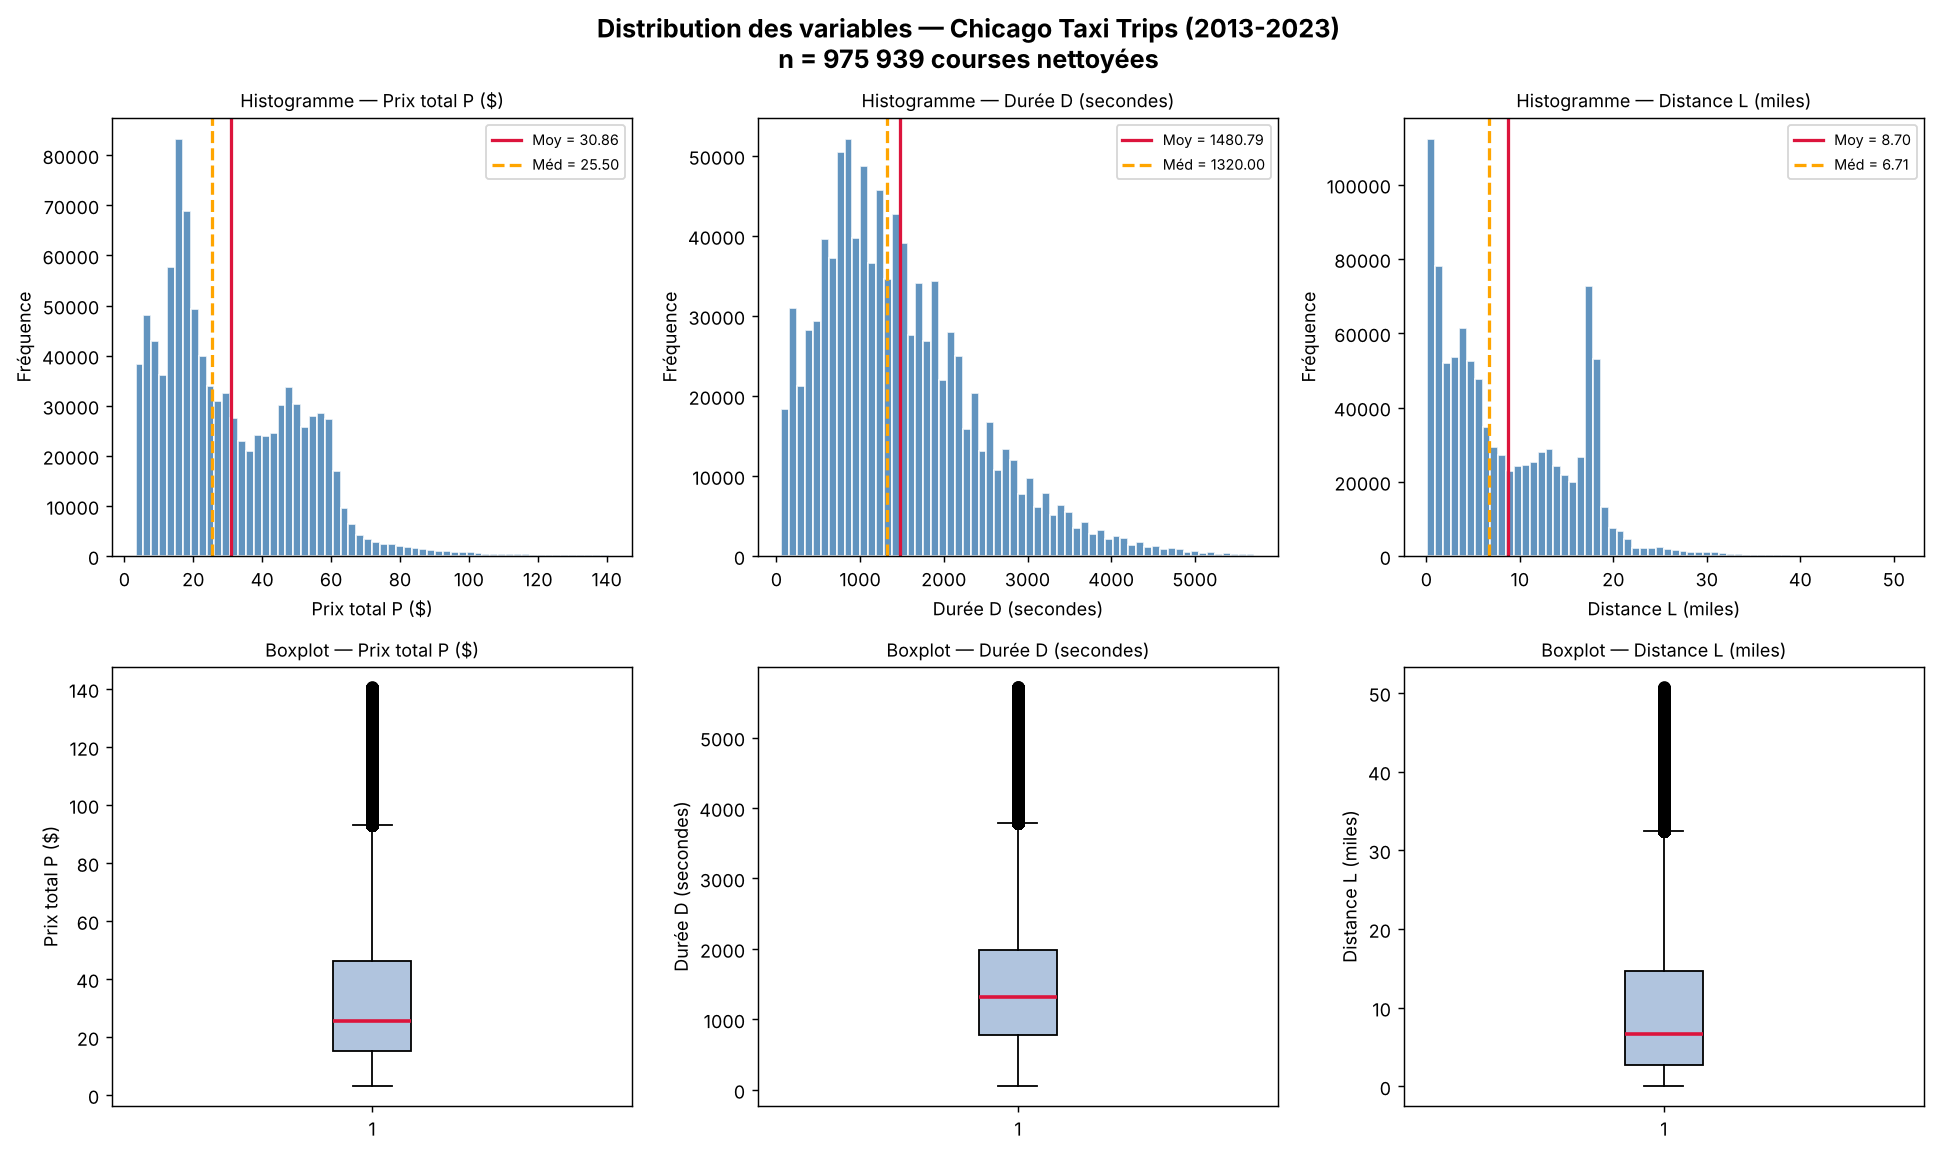
\includegraphics[width=\linewidth]{fig01_distributions.png}
\caption{Histogrammes et boxplots de $P$ (trip\_total), $D$ (trip\_seconds) et $L$ (trip\_miles)}
\end{figure}

\subsection{Évolution annuelle}

Le tableau~\ref{tab:annuel} et la figure~\ref{fig:annuel} montrent l'évolution des moyennes annuelles.
Le prix moyen passe de 19{,}79\,\$ en 2013 à 34{,}87\,\$ en 2019, avec une rupture nette entre 2015
(22{,}63\,\$) et 2016 (29{,}98\,\$) : la distance moyenne passe dans le même temps de 6{,}93 à
9{,}25 miles, ce qui traduit une baisse de la part des courses courtes. L'année 2020 marque un creux
(31{,}33\,\$), puis les valeurs de 2021 reviennent au niveau de 2019.

\begin{table}[H]
\centering
\caption{Nombre de courses retenues et moyennes annuelles de $P$, $D$ et $L$}
\label{tab:annuel}
\begin{tabular}{lrrrr}
\toprule
\headrowcolor \thead{Année} & \thead{$n$} & \thead{$\bar P$ (\$)} & \thead{$\bar D$ (s)} & \thead{$\bar L$ (miles)} \\
\midrule
2013 & 39\,664 & 19{,}79 & 1\,144{,}1 & 5{,}28 \\
2014 & 87\,854 & 20{,}57 & 1\,223{,}5 & 6{,}29 \\
2015 & 82\,820 & 22{,}63 & 1\,340{,}0 & 6{,}93 \\
2016 & 100\,102 & 29{,}98 & 1\,430{,}3 & 9{,}25 \\
2017 & 95\,871 & 32{,}40 & 1\,542{,}5 & 9{,}27 \\
2018 & 96\,324 & 33{,}79 & 1\,613{,}0 & 9{,}44 \\
2019 & 94\,601 & 34{,}87 & 1\,644{,}6 & 9{,}40 \\
2020 & 95\,266 & 31{,}33 & 1\,466{,}4 & 8{,}66 \\ \midrule
2021 & 94\,792 & 34{,}51 & 1\,536{,}3 & 9{,}54 \\ \midrule
2022 & 93\,720 & 35{,}27 & 1\,546{,}0 & 9{,}52 \\
2023 & 94\,925 & 36{,}17 & 1\,570{,}3 & 9{,}65 \\
\bottomrule
\end{tabular}
\end{table}

\begin{figure}[H]
\centering
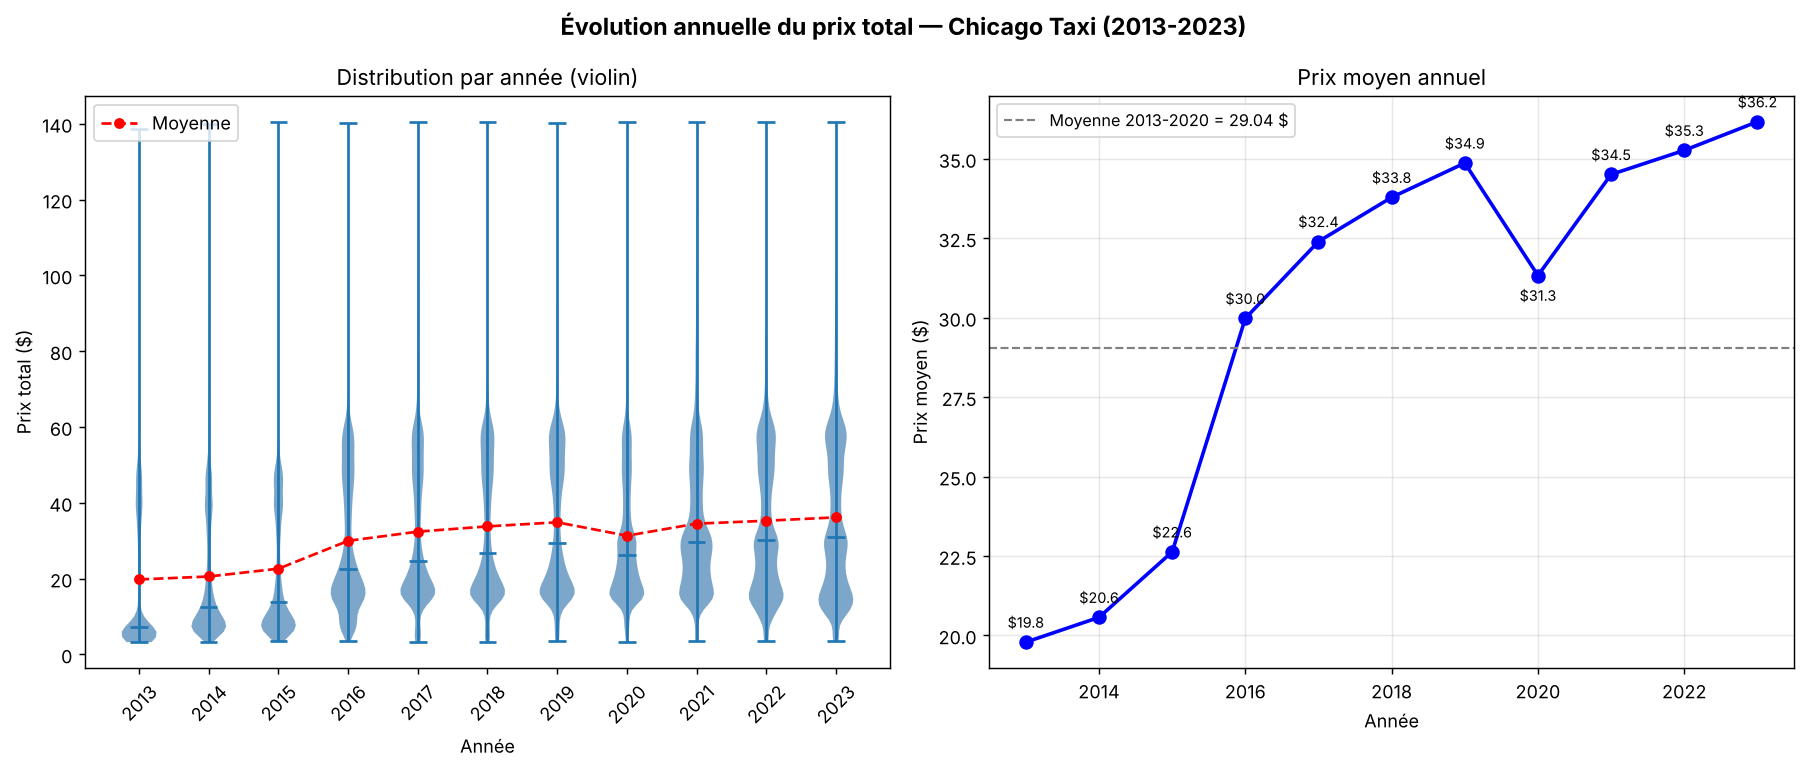
\includegraphics[width=\linewidth]{fig02_evolution_annuelle.png}
\caption{Évolution annuelle du prix de 2013 à 2023 (violin plots et prix moyen annuel)}
\label{fig:annuel}
\end{figure}

%================= 4 =================
\section{Méthodologie}

Le pipeline suivi est :
\[
\textbf{Collecte} \longrightarrow \textbf{Prétraitement} \longrightarrow \textbf{Transformation}
\longrightarrow \textbf{Analyse} \longrightarrow \textbf{Visualisation}
\]

\subsection{Question 1 --- Test t de Student}

Pour tester si la moyenne d'une variable $X \in \{P, D, L\}$ diffère entre la période de référence et
l'échantillon test, on utilise le \textbf{test $t$ à un échantillon bilatéral} :
\[
H_0 : \mu_{\text{test}} = \mu_{\text{ref}} \qquad \text{vs} \qquad H_1 : \mu_{\text{test}} \neq \mu_{\text{ref}}
\]
La statistique de test est :
\[
t = \frac{\bar X_{\text{test}} - \mu_{\text{ref}}}{s_{\text{test}} / \sqrt{n_{\text{test}}}} \quad\sim\quad t(n_{\text{test}} - 1)
\]
On rejette $H_0$ si $|t| > t_{\alpha/2,\,n-1}$, c'est-à-dire si la p-valeur est inférieure à $\alpha = 0{,}05$.

\textbf{Justification :} la moyenne 2013--2020, calculée sur 692\,502 courses, sert de valeur de référence
$\mu_{\text{ref}}$. Le théorème central limite garantit la normalité de $\bar X$ pour $n > 30$ (ici
$n = $ 94\,792).

\textbf{Compléments :}
\begin{itemize}
  \item La référence étant elle-même un échantillon, le résultat est vérifié par un \textbf{test $t$ de Welch}
        à deux échantillons (2021 vs 2013--2020), qui n'impose pas l'égalité des variances.
  \item Avec près de $10^5$ observations, un écart très faible suffit à rejeter $H_0$. L'importance pratique de
        l'écart est donc mesurée par le \textbf{$d$ de Cohen} :
        $d = (\bar X_{2021} - \bar X_{\text{ref}}) / s_p$, où $s_p$ est l'écart-type combiné
        ($|d| < 0{,}2$ : effet négligeable ; $0{,}2$ à $0{,}5$ : faible ; $0{,}5$ à $0{,}8$ : moyen).
  \item Pour séparer l'effet de l'année 2021 de la tendance de long terme, 2021 est aussi comparée à 2019,
        dernière année avant la pandémie.
\end{itemize}

\subsection{Question 2 --- Corrélation et Régression linéaire}

La \textbf{corrélation de Pearson} mesure la force de la liaison linéaire entre $P$ et chaque variable
explicative :
\[
r(P, X) = \frac{\sum_i (P_i - \bar P)(X_i - \bar X)}{\sqrt{\sum_i (P_i - \bar P)^2} \cdot \sqrt{\sum_i (X_i - \bar X)^2}}
\]
La \textbf{régression linéaire simple} $P = \beta_0 + \beta_1 X + \varepsilon$ est estimée par moindres carrés
ordinaires (MCO). La \textbf{régression multiple} $P = \beta_0 + \beta_1 L + \beta_2 D + \varepsilon$ combine les
deux variables.

\textbf{Justification :} les variables sont continues et les nuages de points révèlent une tendance linéaire.
Le $R^2$ quantifie la part de variance du prix expliquée par le modèle.

\subsection{Question 3 --- ANOVA, test post-hoc et corrélation par plage horaire}

La journée est divisée en 6 tranches de 4 heures : [00h--04h[, [04h--08h[, [08h--12h[, [12h--16h[,
[16h--20h[, [20h--00h[. L'\textbf{ANOVA à un facteur} teste l'égalité des moyennes de $P$ entre les 6 groupes :
\[
H_0 : \mu_1 = \mu_2 = \cdots = \mu_6 \qquad \text{vs} \qquad H_1 : \exists\, i \neq j,\ \mu_i \neq \mu_j
\]
La taille d'effet est mesurée par $\eta^2 = SC_{\text{inter}} / SC_{\text{totale}}$, part de la variance du prix
expliquée par la plage horaire.

\textbf{Test post-hoc de Bonferroni :} l'ANOVA indique seulement qu'au moins un groupe diffère. Pour identifier
\textit{quelles} plages diffèrent significativement entre elles, on effectue des tests $t$ par paires avec
correction de Bonferroni ($\alpha_{\text{corr}} = 0{,}05/15 \approx 0{,}0033$). Ceci permet d'identifier
formellement la plage de pointe.

La corrélation de Pearson $r(P, \text{slot})$ teste la tendance linéaire monotone du prix en fonction du
numéro de plage.

\textbf{Justification :} l'ANOVA évite l'inflation du risque d'erreur de type I inhérente aux tests $t$ par
paires multiples. La correction de Bonferroni contrôle le taux d'erreur global.

%================= 5 =================
\section{Résultats et Interprétation}

\subsection{\texorpdfstring{Question 1 : Test d'hypothèse sur la moyenne de $P$, $D$ et $L$ ($\alpha = 5\,\%$)}{Question 1 : Test d'hypothèse sur la moyenne de P, D et L}}

\begin{table}[H]
\centering
\small
\caption{Résultats du test $t$ bilatéral ($\alpha = 5\,\%$) --- 2021 vs 2013--2020}
\label{tab:q1}
\setlength{\tabcolsep}{4.5pt}
\begin{tabular}{lrrrrrrr}
\toprule
\headrowcolor \thead{Variable} & \thead{$\mu_{\text{ref}}$} & \thead{$\bar X_{2021}$} & \thead{$t$} & \thead{p-valeur}
 & \thead{$t$ Welch} & \thead{$d$} & \thead{Variation} \\
\midrule
$P$ (trip\_total, \$) & 29{,}04 & 34{,}51 & $+$87{,}05 & $\approx 0$ & $+$81{,}55 & 0{,}28 & $+$18{,}8\,\% \\
$D$ (trip\_seconds, s) & 1\,452{,}1 & 1\,536{,}3 & $+$32{,}47 & $5{,}04 \times 10^{-230}$ & $+$29{,}69 & 0{,}09 & $+$5{,}8\,\% \\
$L$ (trip\_miles) & 8{,}34 & 9{,}54 & $+$55{,}41 & $\approx 0$ & $+$51{,}66 & 0{,}17 & $+$14{,}4\,\% \\
\midrule
\multicolumn{8}{l}{\textbf{Décision :} rejeter $H_0$ pour les trois variables (p-valeur $\ll \alpha = 0{,}05$)} \\
\bottomrule
\end{tabular}
\end{table}

Les trois variables présentent un écart statistiquement significatif en 2021 par rapport à la référence
2013--2020, confirmé par le test de Welch :
\begin{itemize}
  \item \textbf{Prix ($P$) :} la moyenne passe de 29{,}04\,\$ à 34{,}51\,\$, soit $+$5{,}47\,\$
        ($+$18{,}8\,\%), avec $t = $ 87{,}05. L'effet est \textbf{faible} ($d = $ 0{,}28).
  \item \textbf{Durée ($D$) :} la durée moyenne passe de 1\,452{,}1\,s à 1\,536{,}3\,s, soit $+$84{,}3\,s
        ($+$5{,}8\,\%), avec $t = $ 32{,}47 et $p = $ $5{,}04 \times 10^{-230}$. L'effet est \textbf{négligeable} ($d = $ 0{,}09).
  \item \textbf{Distance ($L$) :} la distance moyenne passe de 8{,}34 à 9{,}54 miles, soit $+$1{,}20 mile
        ($+$14{,}4\,\%), avec $t = $ 55{,}41. L'effet est \textbf{négligeable} ($d = $ 0{,}17).
\end{itemize}

\textbf{Interprétation :} la significativité s'explique en grande partie par la taille des échantillons ;
les tailles d'effet restent faibles. Surtout, la référence 2013--2020 mélange des années très différentes :
le prix moyen passe de 19{,}79\,\$ en 2013 à 34{,}87\,\$ en 2019 (tableau~\ref{tab:annuel}). La hausse
observée en 2021 traduit donc d'abord la \textbf{tendance de long terme}, et non un effet propre à
l'année 2021. Le tableau~\ref{tab:q19} le confirme en comparant 2021 à 2019.

\begin{table}[H]
\centering
\small
\caption{Analyse complémentaire --- 2021 vs 2019 (test de Welch, $n_{2019} = $ 94\,601, $n_{2021} = $ 94\,792)}
\label{tab:q19}
\begin{tabular}{lrrrrrr}
\toprule
\headrowcolor \thead{Variable} & \thead{$\bar X_{2019}$} & \thead{$\bar X_{2021}$} & \thead{Variation} & \thead{$t$} & \thead{p-valeur} & \thead{$d$} \\
\midrule
$P$ (trip\_total, \$) & 34{,}87 & 34{,}51 & $-$1{,}0\,\% & $-$3{,}99 & $6{,}64 \times 10^{-5}$ & $-$0{,}018 \\
$D$ (trip\_seconds, s) & 1\,644{,}6 & 1\,536{,}3 & $-$6{,}6\,\% & $-$27{,}11 & $1{,}38 \times 10^{-161}$ & $-$0{,}125 \\
$L$ (trip\_miles) & 9{,}40 & 9{,}54 & $+$1{,}5\,\% & $+$4{,}46 & $8{,}32 \times 10^{-6}$ & $+$0{,}020 \\
\bottomrule
\end{tabular}
\end{table}

Par rapport à 2019, le prix moyen de 2021 est quasiment identique ($-$1{,}0\,\%, $d = $ $-$0{,}018) et la
distance aussi ($+$1{,}5\,\%, $d = $ $+$0{,}020). Le seul changement notable est une \textbf{baisse de la durée}
($-$6{,}6\,\%, $d = $ $-$0{,}125) pour des distances comparables, ce qui est compatible avec une circulation
moins dense en 2021, pendant la pandémie de COVID-19. Ces écarts restent toutefois d'ampleur négligeable.

\subsection{Question 2 : Relation entre Prix, Longueur et Durée}

\subsubsection{Corrélations de Pearson}
\[
r(P, L) = 0{,}845 \quad (p \approx 0) \qquad\qquad r(P, D) = 0{,}714 \quad (p \approx 0)
\]
La liaison entre $P$ et $L$ est \textbf{forte} ($r = $ 0{,}845) ; celle entre $P$ et $D$ est \textbf{modérée à
forte} ($r = $ 0{,}714). Les p-valeurs sont en sous-dépassement numérique ($< 2{,}2 \times 10^{-308}$), ce qui
confirme une significativité extrême pour $n = $ 975\,939. Les deux variables explicatives sont elles-mêmes
corrélées : $r(L, D) = $ 0{,}659.

\subsubsection{Modèles de régression (MCO sur 975\,939 courses)}

\begin{table}[H]
\centering
\caption{Résultats des modèles de régression linéaire}
\label{tab:q2}
\begin{tabular}{llr}
\toprule
\headrowcolor \thead{Modèle} & \thead{Équation estimée (MCO)} & \thead{$R^2$} \\
\midrule
$P \sim L$ & $\hat P = 9{,}73 + 2{,}430 \cdot L$ & 0{,}714 \\
$P \sim D$ & $\hat P = 8{,}12 + 0{,}01536 \cdot D$ & 0{,}510 \\
$P \sim L + D$ & $\hat P = 5{,}45 + 1{,}902 \cdot L + 0{,}005994 \cdot D$ & \textbf{0{,}758} \\
\bottomrule
\end{tabular}
\end{table}

La régression simple $P \sim L$ explique \textbf{71{,}4\,\%} de la variance du prix ; la durée seule
($P \sim D$) en explique 51{,}0\,\%. L'ajout de $D$ dans le modèle $P \sim L + D$ porte le $R^2$ à
\textbf{0{,}758}, soit un gain de 4{,}4 points de pourcentage : distance et durée sont deux facteurs
complémentaires dans la tarification. L'erreur quadratique moyenne du modèle multiple est de 9{,}86\,\$.

\textbf{Interprétation :}
\begin{itemize}
  \item Dans le modèle simple, chaque mile supplémentaire augmente le prix de 2{,}43\,\$ (facteur dominant).
  \item La durée seule contribue 0{,}01536\,\$ par seconde ($\approx$ 0{,}92\,\$/min).
  \item Dans le modèle multiple, le coefficient de $L$ (1{,}90\,\$/mile) et celui de $D$ (0{,}36\,\$/min) sont
        plus faibles que dans les modèles simples, car $L$ et $D$ sont corrélées : une partie de l'effet de la
        durée est déjà portée par la distance. Le terme en $D$ capte la tarification à l'attente
        (embouteillages).
  \item L'intercept (5{,}45\,\$) correspond aux frais fixes de prise en charge (\textit{flag drop}), auxquels
        s'ajoutent les pourboires et suppléments inclus dans \texttt{trip\_total}.
\end{itemize}

\begin{figure}[H]
\centering
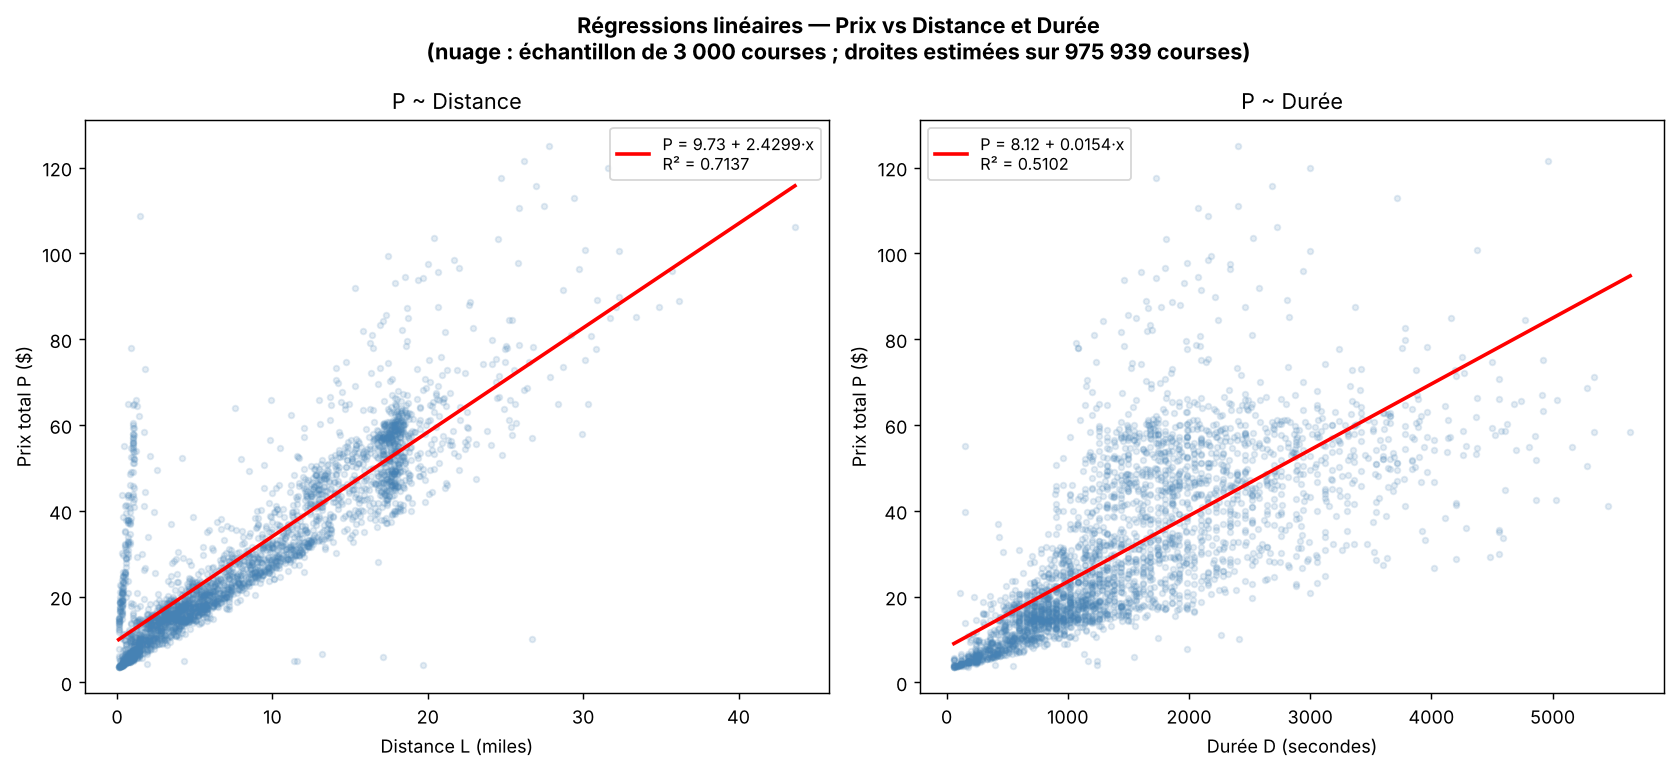
\includegraphics[width=\linewidth]{fig03_regression.png}
\caption{Nuages de points (échantillon de 3\,000 courses) et droites de régression : $P \sim L$ (gauche) et
$P \sim D$ (droite)}
\end{figure}

\subsection{Question 3 : Plages horaires et plage de pointe}

\begin{table}[H]
\centering
\caption{Prix moyen et volume de courses par plage horaire}
\label{tab:q3}
\begin{tabular}{lrrrr}
\toprule
\headrowcolor \thead{Plage horaire} & \thead{Courses} & \thead{Part} & \thead{Prix moyen (\$)} & \thead{Écart-type (\$)} \\
\midrule
{[}00h--04h{[} & 69\,750 & 7{,}2\,\% & \textbf{24{,}69} & 18{,}78 \\
{[}04h--08h{[} & 72\,008 & 7{,}4\,\% & 32{,}32 & 19{,}15 \\
{[}08h--12h{[} & 178\,403 & 18{,}3\,\% & 30{,}72 & 20{,}02 \\
{[}12h--16h{[} & 226\,644 & 23{,}2\,\% & \textbf{32{,}95} & 20{,}03 \\
{[}16h--20h{[} & \textbf{254\,812} & 26{,}1\,\% & 30{,}73 & 20{,}05 \\
{[}20h--00h{[} & 174\,322 & 17{,}9\,\% & 30{,}38 & 20{,}32 \\
\midrule
\multicolumn{5}{l}{\textbf{ANOVA :} $F = $ 1\,936{,}64, $p \approx 0$, $\eta^2 = $ 0{,}0098 \quad $\Rightarrow$ Rejet de $H_0$} \\
\multicolumn{5}{l}{\textbf{Corrélation :} $r(P, \text{slot}) = $ 0{,}032, $p = $ $8{,}17 \times 10^{-219}$} \\
\bottomrule
\end{tabular}
\end{table}

\begin{figure}[H]
\centering
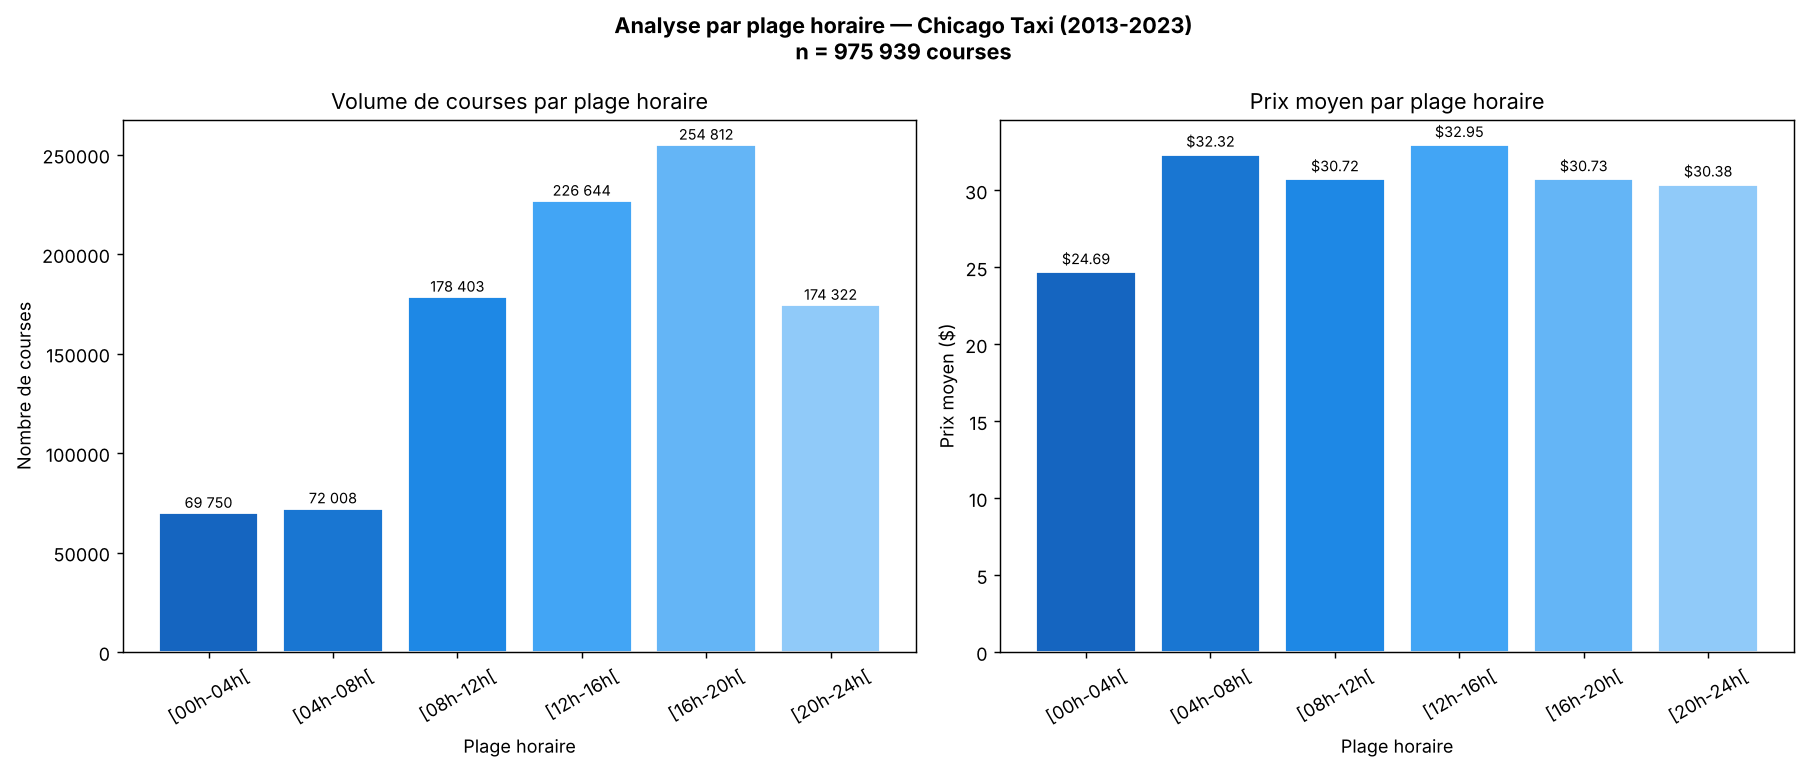
\includegraphics[width=\linewidth]{fig04_plages_horaires.png}
\caption{Volume de courses (gauche) et prix moyen (droite) par plage horaire de 4\,h}
\end{figure}

L'ANOVA ($F = $ 1\,936{,}64, $p \ll 0{,}05$) rejette $H_0$ : les moyennes de prix diffèrent significativement entre
les 6 plages. Cependant, $\eta^2 = $ 0{,}0098 : la plage horaire n'explique qu'environ 1{,}0\,\% de la
variance du prix, qui dépend avant tout de la distance (question~2).

La plage \textbf{{[}16h--20h{[}} concentre le plus grand volume de courses (254\,812, soit 26{,}1\,\% du total) :
c'est la \textbf{plage de pointe} en termes d'activité (retours domicile-travail). Le prix moyen est le plus élevé
en {[}12h--16h{[} (32{,}95\,\$) et minimal la nuit, en {[}00h--04h{[} (24{,}69\,\$).

La corrélation linéaire $r(P, \text{slot}) = $ 0{,}032 est très faible mais significative
($p = $ $8{,}17 \times 10^{-219}$) : la relation entre le prix et la plage n'est \textbf{pas linéaire monotone}, le prix
n'augmente pas régulièrement avec l'heure. L'ANOVA est donc plus appropriée que la corrélation seule.

\subsection{Test post-hoc de Bonferroni}

L'ANOVA ayant rejeté $H_0$, il est nécessaire de déterminer quelles paires de plages horaires diffèrent
significativement. On applique le \textbf{test post-hoc de Bonferroni} : pour chacune des $\binom{6}{2} = 15$
paires, un test $t$ de Welch (variances inégales) est réalisé, puis la p-valeur brute est corrigée par
multiplication par 15 :
\[
p_{\text{adj}} = \min(p_{\text{brut}} \times 15,\; 1), \qquad \alpha_{\text{adj}} = \frac{0{,}05}{15} \approx 0{,}0033.
\]

\begin{table}[H]
\centering
\small
\caption{Résultats du test post-hoc de Bonferroni --- 15 paires de plages horaires}
\label{tab:posthoc}
\begin{tabular}{llrrrc}
\toprule
\headrowcolor \thead{Plage $i$} & \thead{Plage $j$} & \thead{$\Delta\bar P$ (\$)} & \thead{$t$} & \thead{$p_{\text{adj}}$} & \thead{Sig.} \\
\midrule
{[}00h--04h{[} & {[}04h--08h{[} & $-$7{,}64 & $-$75{,}81 & $\approx 0$ & *** \\
{[}00h--04h{[} & {[}08h--12h{[} & $-$6{,}04 & $-$70{,}65 & $\approx 0$ & *** \\
{[}00h--04h{[} & {[}12h--16h{[} & $-$8{,}26 & $-$100{,}01 & $\approx 0$ & *** \\
{[}00h--04h{[} & {[}16h--20h{[} & $-$6{,}04 & $-$74{,}18 & $\approx 0$ & *** \\
{[}00h--04h{[} & {[}20h--00h{[} & $-$5{,}69 & $-$66{,}07 & $\approx 0$ & *** \\
\midrule
{[}04h--08h{[} & {[}08h--12h{[} & $+$1{,}60 & $+$18{,}66 & $2{,}11 \times 10^{-76}$ & *** \\
{[}04h--08h{[} & {[}12h--16h{[} & $-$0{,}63 & $-$7{,}56 & $5{,}90 \times 10^{-13}$ & *** \\
{[}04h--08h{[} & {[}16h--20h{[} & $+$1{,}59 & $+$19{,}52 & $1{,}43 \times 10^{-83}$ & *** \\
{[}04h--08h{[} & {[}20h--00h{[} & $+$1{,}94 & $+$22{,}50 & $9{,}49 \times 10^{-111}$ & *** \\
\midrule
{[}08h--12h{[} & {[}12h--16h{[} & $-$2{,}22 & $-$35{,}10 & $3{,}14 \times 10^{-268}$ & *** \\
\rowcolor{nsrow} {[}08h--12h{[} & {[}16h--20h{[} & $-$0{,}00 & $-$0{,}06 & $1$ & n.s. \\
{[}08h--12h{[} & {[}20h--00h{[} & $+$0{,}35 & $+$5{,}08 & $5{,}63 \times 10^{-6}$ & *** \\
\midrule
{[}12h--16h{[} & {[}16h--20h{[} & $+$2{,}22 & $+$38{,}38 & $\approx 0$ & *** \\
{[}12h--16h{[} & {[}20h--00h{[} & $+$2{,}57 & $+$39{,}95 & $\approx 0$ & *** \\
\midrule
{[}16h--20h{[} & {[}20h--00h{[} & $+$0{,}35 & $+$5{,}56 & $4{,}15 \times 10^{-7}$ & *** \\
\bottomrule
\multicolumn{6}{l}{\footnotesize *** $p_{\text{adj}} < 0{,}001$ \quad n.s. : non significatif \quad
$\Delta\bar P = \bar P_i - \bar P_j$ \quad Test $t$ de Welch bilatéral, $n = $ 975\,939}
\end{tabular}
\end{table}

\begin{figure}[H]
\centering
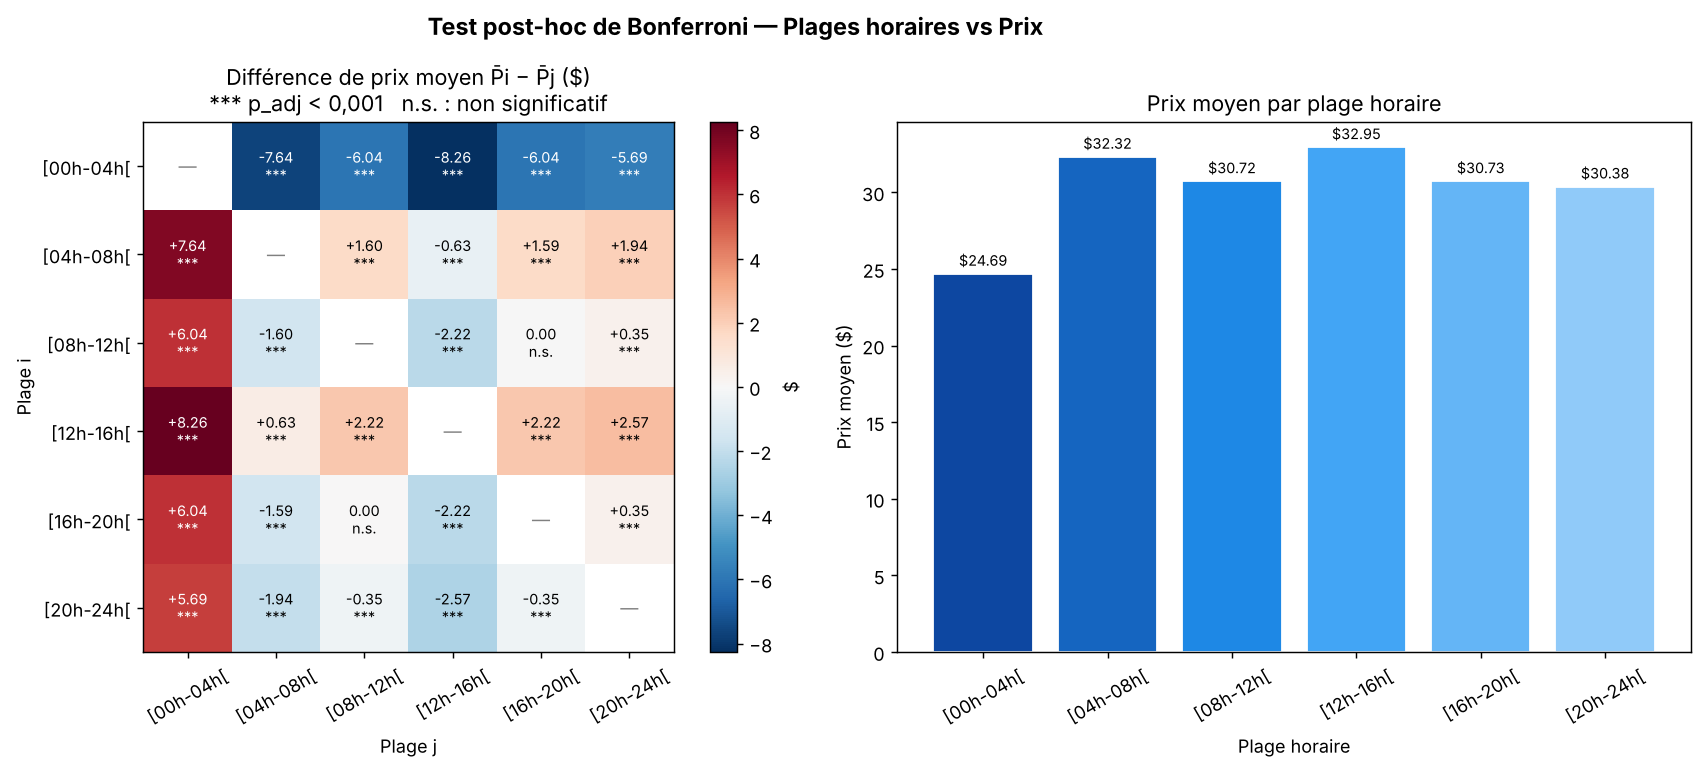
\includegraphics[width=\linewidth]{fig05_posthoc_bonferroni.png}
\caption{Matrice des différences de prix moyen (gauche) et prix moyen par plage (droite) --- test post-hoc de Bonferroni}
\end{figure}

\textbf{Résultat :} \textbf{14 paires sur 15} sont significativement différentes après correction. Plusieurs
points ressortent :
\begin{itemize}
  \item La plage [00h--04h[ est isolée : son prix moyen (24{,}69\,\$) est inférieur à toutes les autres plages
        d'au moins 5{,}69\,\$ (écart maximal de 8{,}26\,\$ avec [12h--16h[).
  \item La plage [12h--16h[ affiche le prix moyen le plus élevé (32{,}95\,\$), significativement supérieur à
        toutes les autres ($p_{\text{adj}} \ll 0{,}05$).
  \item Les plages [08h--12h[ et [16h--20h[ \textbf{ne diffèrent pas} significativement
        ($\Delta\bar P = $ $-$0{,}004\,\$, $p_{\text{adj}} = 1$) : leurs prix moyens sont identiques.
  \item Les autres petites différences (ex. [08h--12h[ vs [20h--00h[ : $\Delta = $ $+$0{,}35\,\$) restent
        significatives, ce qui s'explique par la taille d'échantillon exceptionnelle ($n \approx 10^6$) et la
        puissance statistique très élevée qui en découle.
\end{itemize}

%================= 6 =================
\section{Conclusion}

Cette étude sur 975\,939 courses de taxi de Chicago (2013--2023) met en évidence trois résultats principaux :
\begin{enumerate}
  \item \textbf{Test d'hypothèse (Q1) :} les moyennes de $P$, $D$ et $L$ en 2021 diffèrent significativement de
        la référence 2013--2020 : prix $+$18{,}8\,\% ($t = $ 87{,}05), durée $+$5{,}8\,\% ($t = $ 32{,}47),
        distance $+$14{,}4\,\% ($t = $ 55{,}41). Les tailles d'effet sont toutefois faibles ($d \le$ 0{,}28),
        et la comparaison avec 2019 montre que les niveaux de 2021 sont proches de ceux d'avant la pandémie
        (prix $-$1{,}0\,\%). La hausse reflète donc surtout la tendance de long terme 2013--2019 ; le seul effet
        propre à 2021 est une durée plus courte à distance égale.
  \item \textbf{Régression (Q2) :} le prix est fortement corrélé à la distance ($r = $ 0{,}845, $R^2 = $ 0{,}714).
        La durée est un facteur complémentaire ($r = $ 0{,}714). Le modèle multiple donne $R^2 = $ 0{,}758 :
        \[ \hat P \approx 5{,}45 + 1{,}902 \cdot L + 0{,}005994 \cdot D \]
        La tarification repose principalement sur la distance (1{,}90\,\$/mile), complétée par un tarif horaire
        (0{,}36\,\$/min) qui capte les embouteillages.
  \item \textbf{Plages horaires (Q3) :} l'ANOVA ($F = $ 1\,936{,}64, $p \ll 0{,}05$) confirme des différences
        significatives entre les 6 plages, mais d'ampleur limitée ($\eta^2 = $ 0{,}0098). La plage
        {[}16h--20h{[} est la plage de pointe en volume (254\,812 courses, 26{,}1\,\%) et {[}12h--16h{[} la plage au
        prix maximal (32{,}95\,\$). La plage nocturne [00h--04h[ a un prix significativement inférieur à toutes
        les autres (24{,}69\,\$). Le test de Bonferroni montre que 14 paires sur 15 diffèrent ; seules
        [08h--12h[ et [16h--20h[ ont des prix équivalents. La corrélation $r(P, \text{slot}) = $ 0{,}032 confirme
        que la variation du prix selon l'heure n'est pas monotone.
\end{enumerate}

\subsection{Limites de l'étude}

\begin{itemize}
  \item \textbf{Échantillonnage :} l'étude porte sur un échantillon d'environ 108\,000 courses par an, et non sur
        la population complète. En 2013, 64\,\% des courses ont été éliminées (distance ou durée non
        renseignée), il n'en reste que 39\,664 : les premières années sont moins bien représentées.
  \item \textbf{Référence hétérogène :} la période 2013--2020 regroupe des années dont les niveaux de prix sont
        très différents ; la comparaison 2021 vs 2019 est plus pertinente pour isoler l'effet de 2021.
  \item \textbf{Significativité et taille d'effet :} avec près d'un million d'observations, presque toute
        différence est significative ; les conclusions s'appuient donc aussi sur $d$ et $\eta^2$.
  \item \textbf{Variable prix :} \texttt{trip\_total} inclut le pourboire, les péages et les suppléments, ce qui
        ajoute de la variabilité non expliquée par $L$ et $D$.
  \item \textbf{Modèle linéaire :} les distributions sont asymétriques et bimodales (trajets vers les aéroports)
        et les résidus ne sont pas homoscédastiques ; la régression est utilisée ici dans un but descriptif.
\end{itemize}

\end{document}
